% Sandia National Laboratories is a multimission laboratory managed and
% operated by National Technology & Engineering Solutions of Sandia, LLC, a
% wholly owned subsidiary of Honeywell International Inc., for the U.S.
% Department of Energy’s National Nuclear Security Administration under
% contract DE-NA0003525.

% Copyright 2002-2020 National Technology & Engineering Solutions of Sandia,
% LLC (NTESS).


\begin{Device}\label{J_DEVICE}

\symbol
{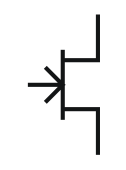
\includegraphics{njfetSymbol}}
{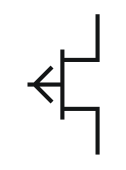
\includegraphics{pjfetSymbol}}

\device
J<name> <drain node> <gate node> <source node> <model name>
+ [area value] [device parameters]

\examples
\begin{alltt}
JIN 100 1 0 JFAST
J13 22 14 23 JNOM 2.0
J1 1 2 0 2N5114
\end{alltt}

\model
\begin{alltt}
.MODEL <model name> NJF [model parameters]
.MODEL <model name> PJF [model parameters]
\end{alltt}

\parameters

\begin{Parameters}

\param{drain node}
Node connected to drain.

\param{gate node}
Node connected to gate.

\param{source node}
 Node connected to source.

\param{source node}
Name of model defined in .MODEL line.

\param{area value}

The \texttt{JFET} is modeled as an intrinsic FET using an ohmic
resistance (\texttt{RD/area}) in series with the drain and another ohmic
resistance (\texttt{RS/area}) in series with the source.  \texttt{area}
is an area factor with a default of \texttt{1}.

\param{device parameters}

Parameters listed in Table~\ref{J_1_Device_Instance_Params} may be
provided as space separated \texttt{<parameter>=<value>} specifications
as needed.  Any number of parameters may be specified.

\end{Parameters}

\comments

The \texttt{JFET} was first proposed and analyzed by Shockley.  The
SPICE- compatible \texttt{JFET} model is an approximation to the
Shockley analysis that employs an adjustable parameter B.  Both the
Shockley formulation and the SPICE approximation are available in Xyce.

\end{Device}

\pagebreak

\paragraph{Device Parameters}
% This table was generated by Xyce:
%   Xyce -doc J 1
%
\index{jfet!device instance parameters}
\begin{DeviceParamTableGenerated}{JFET Device Instance Parameters}{J_1_Device_Instance_Params}
AREA & Device area & m$^{2}$ & 1 \\ \hline
TEMP & Device temperature & -- & Ambient Temperature \\ \hline
\end{DeviceParamTableGenerated}


\paragraph{Model Parameters}
% This table was generated by Xyce:
%   Xyce -doc J 1
%
\index{jfet!device model parameters}
\begin{DeviceParamTableGenerated}{JFET Device Model Parameters}{J_1_Device_Model_Params}
AF & Flicker noise exponent & -- & 1 \\ \hline
B & Doping tail parameter (level 1) & V$^{-1}$ & 1 \\ \hline
BETA & Transconductance parameter & A/V$^{2}$ & 0.0001 \\ \hline
CGD & Zero-bias gate-drain junction capacitance & F & 0 \\ \hline
CGS & Zero-bias gate-source junction capacitance & F & 0 \\ \hline
DELTA & Saturation voltage parrameter (level 2) & V & 0 \\ \hline
FC & Coefficient for forward-bias depletion capacitance & F & 0.5 \\ \hline
IS & Gate junction saturation current & A & 1e-14 \\ \hline
KF & Flicker noise coefficient & -- & 0.05 \\ \hline
LAMBDA & Channel length modulation & V$^{-1}$ & 0 \\ \hline
PB & Gate junction potential & V & 1 \\ \hline
RD & Drain ohmic resistance & $\mathsf{\Omega}$ & 0 \\ \hline
RS & Source ohmic resistance & $\mathsf{\Omega}$ & 0 \\ \hline
TEMPMODEL & Specifies the type of parameter interpolation over temperature & -- & 'NONE' \\ \hline
THETA & Mobility modulation parameter (level 2) & V$^{-1}$ & 0 \\ \hline
TNOM & Nominal device temperature & $^\circ$C & Ambient Temperature \\ \hline
VTO & Threshold voltage & V & -2 \\ \hline
\end{DeviceParamTableGenerated}


\pagebreak

\paragraph{Device Parameters}
% This table was generated by Xyce:
%   Xyce -doc J 2
%
\index{jfet!device instance parameters}
\begin{DeviceParamTableGenerated}{JFET Device Instance Parameters}{J_2_Device_Instance_Params}
AREA & Device area & m$^{2}$ & 1 \\ \hline
TEMP & Device temperature & -- & Ambient Temperature \\ \hline
\end{DeviceParamTableGenerated}


\paragraph{Model Parameters}
% This table was generated by Xyce:
%   Xyce -doc J 2
%
\index{jfet!device model parameters}
\begin{DeviceParamTableGenerated}{JFET Device Model Parameters}{J_2_Device_Model_Params}
AF & Flicker noise exponent & -- & 1 \\ \hline
B & Doping tail parameter (level 1) & V$^{-1}$ & 1 \\ \hline
BETA & Transconductance parameter & A/V$^{2}$ & 0.0001 \\ \hline
CGD & Zero-bias gate-drain junction capacitance & F & 0 \\ \hline
CGS & Zero-bias gate-source junction capacitance & F & 0 \\ \hline
DELTA & Saturation voltage parrameter (level 2) & V & 0 \\ \hline
FC & Coefficient for forward-bias depletion capacitance & F & 0.5 \\ \hline
IS & Gate junction saturation current & A & 1e-14 \\ \hline
KF & Flicker noise coefficient & -- & 0.05 \\ \hline
LAMBDA & Channel length modulation & V$^{-1}$ & 0 \\ \hline
PB & Gate junction potential & V & 1 \\ \hline
RD & Drain ohmic resistance & $\mathsf{\Omega}$ & 0 \\ \hline
RS & Source ohmic resistance & $\mathsf{\Omega}$ & 0 \\ \hline
TEMPMODEL & Specifies the type of parameter interpolation over temperature & -- & 'NONE' \\ \hline
THETA & Mobility modulation parameter (level 2) & V$^{-1}$ & 0 \\ \hline
TNOM & Nominal device temperature & $^\circ$C & Ambient Temperature \\ \hline
VTO & Threshold voltage & V & -2 \\ \hline
\end{DeviceParamTableGenerated}


\paragraph{JFET Level selection}
\Xyce{} supports two JFET models.  LEVEL=1, the default, is the SPICE 3f5
treatment.  This model employs a doping profile parameter B.  When B=1,
the original SPICE square law is exactly implemented, and when B=0.6 the
model is close to that of Shockley.

When LEVEL=2 is selected, the Shockley model is used with some additional physics
effects:  channel length modulation and the effect of gate electric field on
mobility.  An additional parameter, DELTA, is added to the LEVEL 2 model that
allows the user to adjust the saturation voltage.

\paragraph{JFET Power Calculations}
Power dissipated in the transistor is calculated with $I_{D}*V_{DS}+I_{G}*V_{GS}$ where
$I_{D}$ is the drain current, $I_{G}$ is the gate current, $V_{DS}$ is the 
voltage drop between the drain and the source and $V_{GS}$ is the voltage drop 
between the gate and the source. This formula may differ from other simulators,
such as HSPICE and PSpice.
